\chapter{Introduction}
The topic of my project is a device driver for BlueNRG in the Linux kernel.\\
BlueNRG is a Bluetooth Low Energy network coprocessor developed by STMicroelectronics.
Bluetooth is a wireless technology standard for exchanging data over short distances. While exchanging data is the most accurate and popular use case of Bluetooth, the technology has transcended this simple initial purpose. Bluetooth is managed by the Bluetooth Special Interest Group (SIG), which has more than 25,000 member companies in the areas of telecommunication, computing, networking and consumer electronics. Bluetooth technology has found itself to be a perfect fit for many and many short distance communication problems, and has also re invented and improved itself over the years in order to keep up with the market trends. One such monumental change or addition to Bluetooth that is going to feature heavily in this report is Bluetooth Low Energy, a smarter and edgier version of Bluetooth.
\section{Technologies Used}
\subsection{Bluetooth Low Energy} Marketed as \textbf{Bluetooth Smart}) is a wireless personal area network technology designed and marketed by the \textbf{Bluetooth Special Interest Group aimed} at novel applications in the healthcare, fitness, beacons, security, and home entertainment industries. \\
It is part of the Bluetooth \textbf{4.0 specification}. It aims at being a low energy, low cost, low bandwidth, low power and low complexity extensible framework for exchanging data pertaining to various applications fields.
\subsection{BeagleBone Black} The BeagleBoard is a low-power open-source hardware single-board computer produced by Texas Instruments in association with Digi-Key and Newark element14. The BeagleBoard was also designed with open source software development in mind, and as a way of demonstrating the Texas Instrument's OMAP3530 system-on-a-chip. The board was developed by a small team of engineers as an educational board that could be used in colleges around the world to teach open source hardware and software capabilities. It is also sold to the public under the Creative Commons share-alike license. The board was designed using Cadence OrCAD for schematics and Cadence Allegro for PCB manufacturing; no simulation software was used.
\begin{figure}[ht]
	        \centering
	        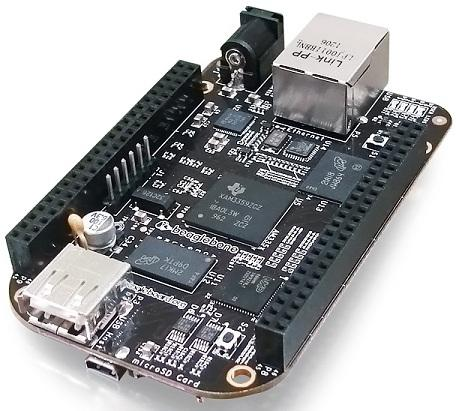
\includegraphics[width=3.5in, height=3in]{images/beaglebone_black.png}
	        \caption{BeagleBone Black}
\end{figure}
\subsection{Raspberry Pi} Raspberry Pi is a series of credit card-sized single-board computers developed in the United Kingdom by the Raspberry Pi Foundation to promote the teaching of basic computer science in schools and developing countries. The original model got way more popular than anticipated, outside of the target market; enthusiasts use it, and the later models, for various uses, such as robotics. Accessories, such as keyboard and mice (not needed for some uses) and even a case, are not included, while planned for; they've frequently been included in unofficial bundles, and later in an official bundle.
\begin{figure}[ht]
        \centering
        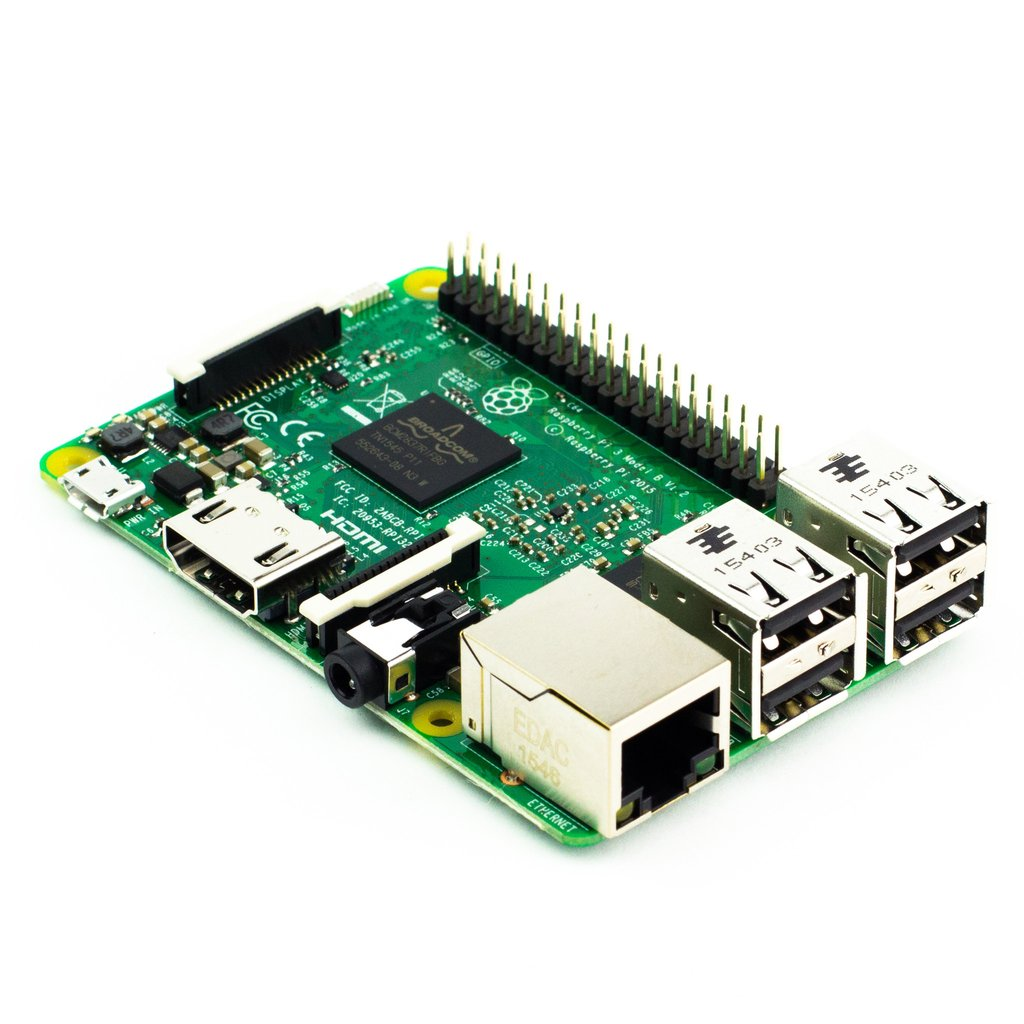
\includegraphics[width=3.5in, height=3in]{images/raspberry_pi.png}
        \caption{Raspberry Pi 3}
\end{figure}
\subsection{Buildroot} Buildroot is a set of Makefiles and patches that simplifies and automates the process of building a complete and bootable Linux environment for an embedded system, while using cross-compilation to allow building for multiple target platforms on a single Linux-based development system. Buildroot can automatically build the required cross-compilation toolchain, create a root file system, compile a Linux kernel image, and generate a boot loader for the targeted embedded system, or it can perform any independent combination of these steps. For example, an already installed cross-compilation toolchain can be used independently, while Buildroot only creates the root file system.
\begin{figure}[ht]
	\centering
        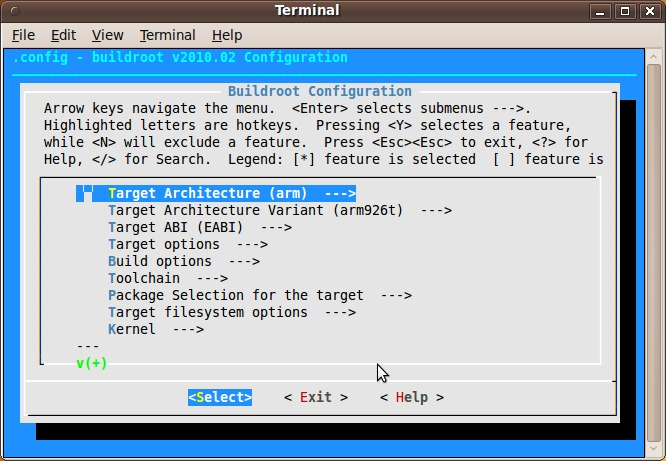
\includegraphics[width=3.5in, height=3in]{images/buildroot.png}
	\caption{Buildroot}
\end{figure}
